\section{Hadronic Jets}
\label{sec:reco:jets}

\indent Energetic partons carrying color charge that are produced in the initial hard scattering will quickly hadronize and then fragment into additional hadrons.  The result is a shower of charged and neutral hadrons referred to as parton shower.  The parton shower leaves a roughly conical energy deposit in the electromagnetic and hadronic calorimeter and multiple associated tracks in the inner tracker.  Some energy may even be deposited in the muon spectrometer if the initial hadron is energetic enough.  This detector signature is referred to as a jet. \\

\indent Identification and reconstruction of hadronic jets is very important for many different detector signatures but especially for our analysis.  Of key importance is the correct reconstruction of the energy of the initial hadron.  The reconstruction of jets and the calibration of the jet's energy is described int he sections \ref{sec:jet:reco} and \ref{sec:jet:calib} below.  Also important is the rejection of jets resulting from proton-proton interactions that are not from the hard scattering and identifying jets resulting from heavy flavour b-quarks described in section \ref{sec:jet:JVT} and \ref{sec:jet:btag}.

\subsection{Hadronic Jet Reconstruction}
\label{sec:jet:reco}

\indent Hadronic jets are reconstructed by clustering energy deposits in the calorimeter.  This procedure involves multiple steps that are described below. \\
\indent First, clusters of energy deposits are formed by clustering all topologically connected calorimeter cells around seed cells that pass the $4\sigma$ signal above noise threshold.  These 3D clusters are referred to as topological clusters (topo-clusters).\cite{jetReco7TeV,jetReco13TeV}  For each cluster, neighboring cells around the seed cell are added to the cluster if they pass $2\sigma$ signal over noise threshold.  Next any cells neighboring any of the cluster cells with above $2\sigma$ signal over noise ratio is also added.  This step is repeated until no neighboring cells pass the $2\sigma$ signal over noise threshold.  At this stage, one last round of neighboring cells is added regardless of the amount of signal to noise ratio in those cells. \\

\indent Topo-clusters are then grouped into jets according to the $\antikt$ algorithm.  The $\antikt$ algorithm groups objects according to the distance measure $d_{ij}$ defined in equation \ref{eqn:antikt} with parameter $p=-1$.  All objects within $d_{ij}$ less then $d_{iB}=k^{2p}_{Ti}$ are grouped into a single jet.  \\

\begin{equation}
d_{ij} = min ( k^{2p}_{Ti}, k^{2p}_{Tj} ) \frac{(\Delta\eta^2_{ij} + \Delta\phi^2_{ij})}{R^2}
\label{eqn:PileupDensity}
\end{equation}

\indent  The algorithm can best be explained by examining an example case.  If a hard object $1$ exists and is surrounded by only soft objects $j$ then $d_{1j}$ equals $k^{2p}_{1j}(\frac{\Delta R^2}{R^2})$ for all $j$ and $\Delta R = \Delta \eta^2 + \Delta \phi^2$.  $d_{1j}$ will always be less then any $d_{ij}$ if both $i$ and $j$ are both soft and have the same $\Delta R$ as $1$ and $j$.  Therefore, the $\antikt$ algorithm effectively groups hard objects first before soft objects.  A perfectly conical jet of radius $R$ will be formed if no other hard objects are found within a cone of $2R$.  If two hard objects exist within $R<\Delta R_{1,2}<2R$ of one another then two jets will be formed with energy cells spit between the two.  If two hard objects exist within $\Delta R_{1,2}<R$ then they will both be grouped to within a single jet. \\

\indent  The $\antikt$ algorithm is both infrared and collinear safe.  Meaning the algorithm is insensitive to the radiation of additional soft particles and the collinear splitting of initial partons.  Additional soft partons do not change the shape of the jets but the jet shape is flexible to accommodate the presence of other hard radiation. \\

\indent ID Tracks are associated with jets according to a {\it ghost association} procedure.\cite{JetAreaGhostAssociate}  Tracks with the same direction and location as real ID tracks but infinitesimally low $\pt$ are allowed to be clustered by the $\antikt$ algorithm.  If these tracks are assigned to the jet by the $\antikt$ algorithm then the real track is associated with the jet.  In this way, we can determine which tracks are associated with the track without disturbing the clustering of calorimeter energy.  The same procedure of clustering infinitesimally low $\pt$ objects is used to determine jet area. \\

\subsection{Jet Calibration and Systematics}
\label{sec:jet:calib}

\indent Both the electromagnetic and hadronic calorimeters on ATLAS are sampling calorimeters.  The energy from the shower deposited in the absorber material is effectively lost because the absorber do not actively record a signal.  Therefore the energy measured using the active material must be scaled up to compensate for this loss.  For this reason and others including leakage of energy outside of the calorimeter edges and deposition of energy below the energy thresholds, reconstructed jets must be calibrated to determine the original hadron's energy.  \\

\indent  A variety of both MC based and data based methods are used to calibrate hadronic jets.  Figure \ref{fig:jetCalibFlow} shows the steps in jet calibration for Run 2.\cite{Calibartion13TeV} \\

\begin{figure}[htb]
  \begin{center}
    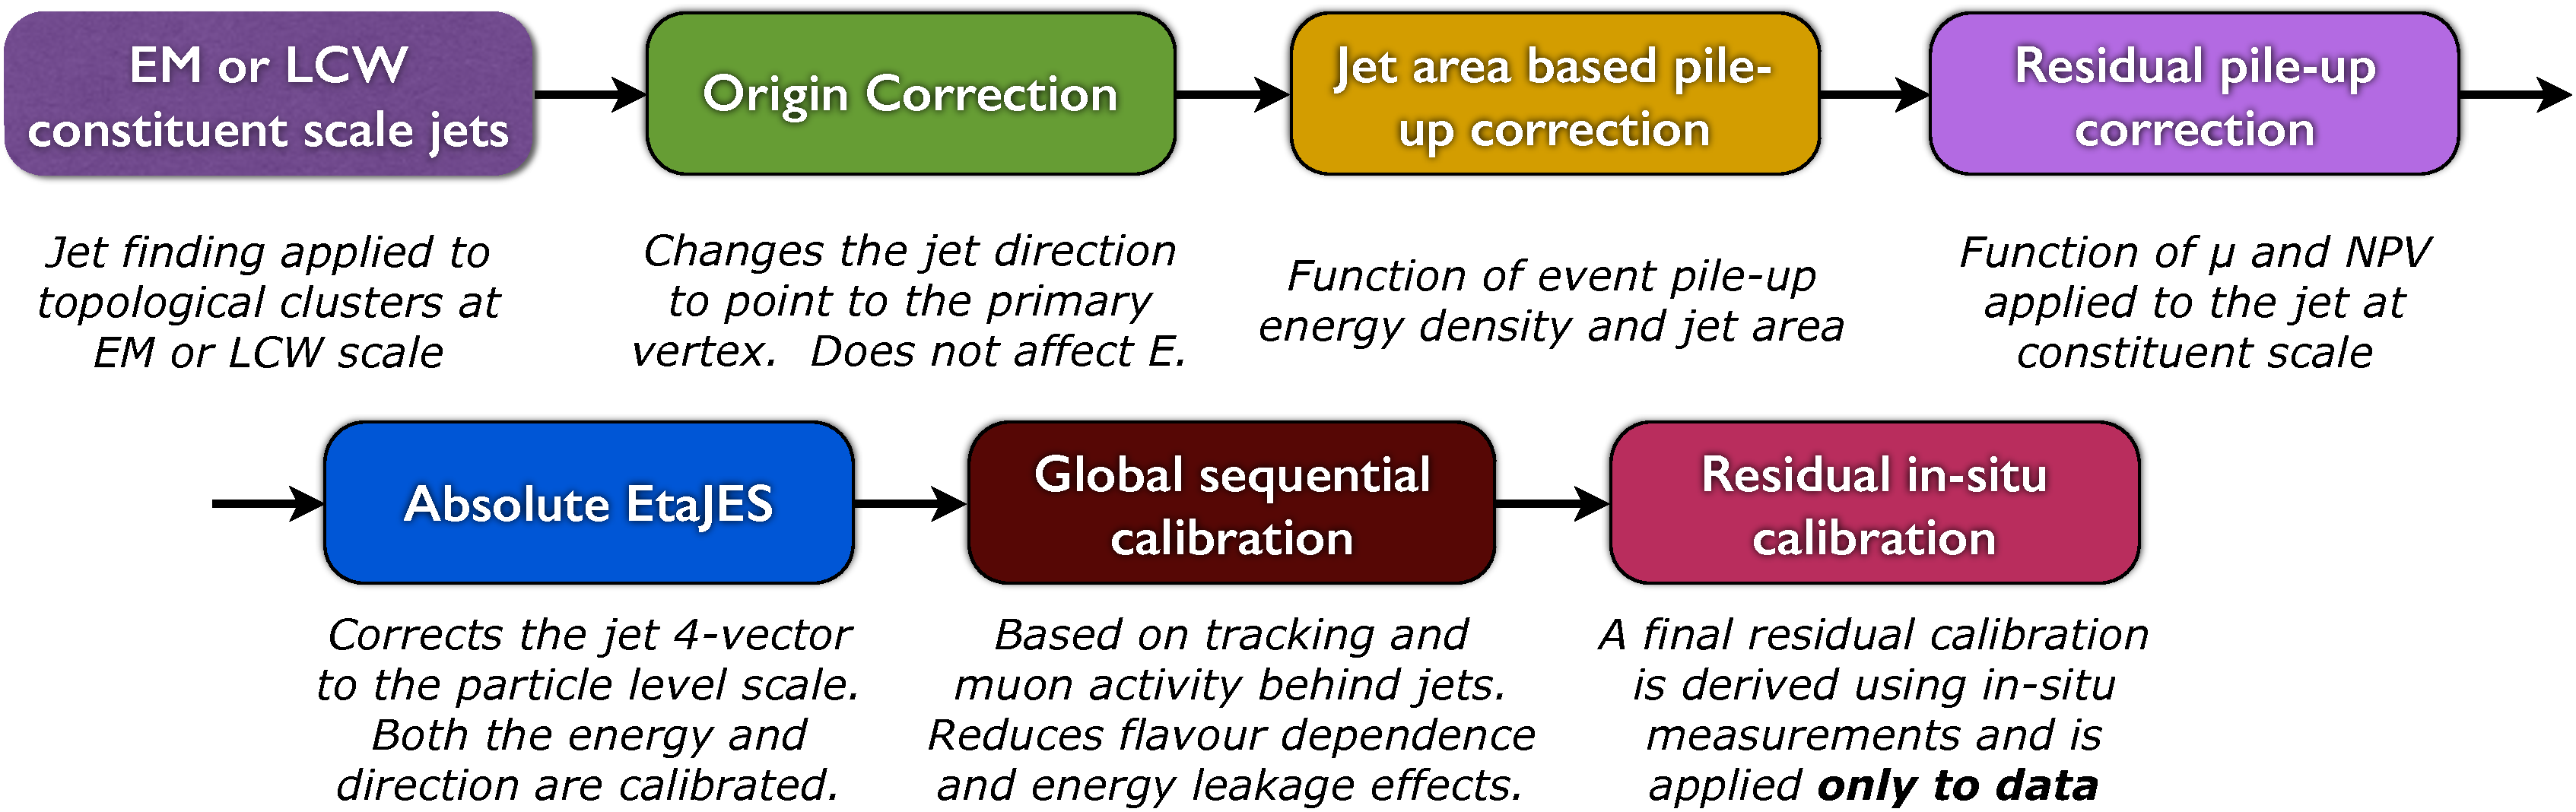
\includegraphics[width=0.85\textwidth]{figures/JetCalib/JetCalibFlow.png}\hspace{0.05\textwidth}
\end{center}
\caption{Flow chart of the steps involved in jet calibration}
\label{fig:jetCalibFlow} 
\end{figure}

\indent First the individual topo-clusters in the jet are calibrated using MC to the energy scale of EM showers.\cite{topoCalib}  This corresponds to the EM calibration scheme.  Next the origin of the reconstructed jet is set to the primary vertex instead of the default detector center. \\

\indent A correction for energy deposited by pileup interactions are then applied.\cite{pileupsub}  The correction is based on the measurement of average energy originating from pileup $\rho$ multiplied by the measured jet area.  The pileup energy density is defined in equation \ref{eqn:PileupDensity} and determined by measuring the median energy density of $R=0.4$ $k_t$ jets found in the central $|\eta|<2.0$ part of the calorimeter.  The $k_t$ algorithm preferentially cluster soft objects first instead of hard objects like the $\antikt$ algorithm and is more sensitive to soft pileup radiation.  No $\pt$ thresholds are applied to the reconstructed $k_t$ jets as we are trying to measure soft objects.  \\

\begin{equation}
\rho=median\{ \frac{p_{T i}^{k_t~jet}}{A_i^{k_t~jet}} \}
\label{eqn:PileupDensity}
\end{equation}

\indent  It is noted that the jet energy response still has a dependence on pileup after this area based correction has been applied.  The sources of this dependence is attributed to the incomplete cancelation of in-time and out-of-time pileup.\cite{JetCalibartion13TeV}  For example, events with a low number of reconstructed vertexes ($N_{PV}$) but in a run with high average number of interactions per bunch crossing ($<\mu>$) may receive relatively large amounts of out-of-time pileup compared to in-time pileup.  This affect is also parameterized using MC by using the constants $\alpha$ and $\beta$.  

\indent The area based pileup energy correction is subtracted along with two other residual corrections.  The total pileup correction to jet $\pt$ is given in equation \ref{pilupCorrection}. \\

\begin{equation}
p_T^{corr} = p_T - \rho \times A - \alpha~\times (N_{PV} - 1 ) - \beta~\times <\mu>
\label{eqn:pilupCorrection}
\end{equation}

\indent In the next step, the jet energy scale (JES) is applied.  JES is a scale factor which relates the reconstructed jet energy with the true jet energy.  JES is calibrated using a number of MC and data driven methods.  The JES is derived from an inclusive jet MC after pileup and origin corrections are applied.  \\

\indent An up to 8 percent difference between the energy responses of gluon and light quark jets remains after the above JES calibration.\cite{JetCalibartion13TeV}  The difference is due to a number of reasons including the factor of 2 difference in color charge between quarks and gluons.  A Global Sequential Correction scheme (GSC) is applied to account for this deference and correct for other detector based issues.\cite{jet_GSC}  GSC corrections uses information on the topology of energy deposits, associated inner detector tracks and activity in the muon spectrometer behind the jet.  ID Tracking information is used to reduce the flavour dependence of the calorimeter response to jets because gluon initiated jets tend to have a wider profile and more tracks. Muon spectrometer information is used to better estimate high energy jets which penetrate the full depth of the calorimeter.  Information on the relative amount of calorimeter energy deposited in specific layers is used to improve the jet energy resolution. \\

\indent Lastly further corrections to the jet energy response are obtained by measuring the balance between jets and some other reference objects such as a photon, a $Z$ boson or other jets directly in data. \cite{JES_ZGamma,JES_dijet}  The $\pt$ balance between jets and the reference objects are measured in data and compared to the MC.  A residual correction is applied by the data over MC ratio based on equation \ref{jet_insitu}.  Systematic uncertainties on the jet energy responses including those on the jet energy scale and jet energy resolution are also derived using these data driven methods. \\

\begin{equation}
\frac{R_{data}}{R_{MC}} = \frac{<p_T^{jet}/p_T^{ref}>_{data}}{<p_T^{jet}/p_T^{ref}>_{MC}}
\label{eqn:jet_insitu}
\end{equation}


\subsection{Pileup Jet Rejection and Jet Vertex Tagger}
\label{sec:jet:JVT}

\indent It is imperative to be able to distinguish between jets origination from the hard scattering interaction (hard scattering jets) and those originating from other proton-proton interactions (pileup jets) in the high luminosity environment.  Pileup jets may originate from both the on average 25 additional p.p. interactions in the same bunch crossing or from interactions in other beam crossing.  We distinguish between the hard scattering jets from pileup jets using a discriminate known as jet vertex tagger (JVT).\cite{JVT} \\

\indent For our analysis we require a jet vertex tagger value greater than 0.59.  This corresponds to a 92 percent efficiency for jets originating from the hard scattering interaction and a 2 percent fake rate from pileup jets, if the jet has $|\eta| < 2.4$ and $\pt < 60 \gev$.\\

\indent The JVT discriminate is based on two variables $\corrJVF$ and $\RpT$ defined in equations \ref{eqn:corrJVF} and \ref{eqn:RpT}.

\begin{equation}
\corrJVF = \frac{\sum_i p_T^{trk_i} (PV_0) }{ \sum_l p_T^{trk_l} (PV_0) + \frac{\sum_{n\ge1} \sum_l p_T^{trk_l} (PV_n) }{k\dot n^{PU}_{trk}} }
\label{eqn:JVF}
\end{equation}

\begin{equation}
\RpT = \frac{\sum_i p_T^{trk_i} (PV_0) }{ p_T^{jet} }
\label{eqn:RpT}
\end{equation}

\indent The $\corrJVF$ variable roughly corresponds to the fraction of a jet's ID track $\pt$ that originate from the hard scattering vertex.  $\sum_i p_T^{trk_i} (PV_0)$ is the sum of all jet's associated track $\pt$ that originate from the primary vertex $PV_0$.  The quantity $p^{PU}_T = \sum_{n\ge1} \sum_l p_T^{trk_l} (PV_n)$ is the total amount of a jet's associated track $\pt$ that originates from pile up interactions.  $p^{PU}_T$ is divided by $k\dot n^{PU}_{trk}$ to correct for the fact that $<k\dot n^{PU}_{trk}>$ will increase linearly with the number of pileup vertexes $n^{PU}_{trk}$.  This makes the variable $\corrJVF$ roughly independent to the number of reconstructed vertexes. The value $k$ is set to an arbitrary $0.01$ and the discriminating power of JVT was found to be independent of the choice of $k$.\\

\indent $\RpT$ is defined as the total track $\pt$ of all associated tracks that originate from the primary vertex $PV_0$ divided by the fully calibrated jet $\pt$. The calibrated jet $\pT$ includes pileup subtraction.  $\RpT$ peaks sharply at zero for pileup jets.  On the other hand, $\RpT$ corresponds to roughly the charged $\pt$ fraction in hard scattering jets.  \\

\indent The JVT discriminate constructs a 2D likelihood based on these variables.   The JVT discriminate determines the probability that a jet will be a hard scattering jet using the k-nearest neighbor (kNN) multivariate technique \cite{TMVA} trained on a $20<\pt<50 \gev$ and $|\eta|<2.4$ MC sample of hard scattering and pileup jets.  The k-nearest neighbor (kNN) algorithm is robust relative to local fluctuations in sparsely populated regions.  \\

\subsection{Identifying Jets Originating from Heavy Flavor Hadrons}
\label{sec:jet:btagging}

